\chapter{Runtimes}
\label{chap:runtimes}

An implementation of the WebAssembly specification \cite{webassemblycommunitygroup_2023_webassembly} is referred to as a WebAssembly runtime or a WebAssembly engine. The initial WebAssembly runtimes were implemented into major browser virtual machines, such as Mozilla's SpiderMonkey and Google's V8 engine. However, as WebAssembly became more mature, it was clear that the characteristics of WebAssembly are also beneficial for other use cases outside of the browser. Therefore, the need for standalone WebAssembly runtimes each with their own characteristics and features emerged. 

This chapter provides an overview of the most popular WebAssembly runtimes, focusing on their distinct characteristics. Additionally, we will delve into the different execution models and explore how they influence the performance of these runtimes. Moreover, we will try to identify the requirements for a \gls{serverless} runtime and compare this approach to something similar like V8 isolates. 

\section{Runtimes Overview}
\label{sec:runtimes-overview}

Table \ref{tab:runtime-overview} presents an overview of the most popular WebAssembly runtimes in each category. The selected runtimes are based on their popularity, support for the WASI standard, and their respective compilation models (JIT, AOT, Interpreter). This selection aims to provide a good representation of the current state of WebAssembly runtimes. 

\begin{table}[htbp]
  \small
  \begin{tabular}{|c|c|c|c|c|c|}
    \hline
    \textbf{Runtime} & \textbf{Embeddable langs.}                                                                                               & \textbf{Architecture}                                                                                                & \textbf{Compiler}                                                         & \textbf{Compilation}                                        & \textbf{Platform}                                                                             \\ \hline
    Wasmtime         & Rust, Python                                                                                                                & \begin{tabular}[c]{@{}c@{}}x86, \\ x86\_64, \\ ARM\end{tabular}                                                      & \begin{tabular}[c]{@{}c@{}}Cranelift, \\ LLVM\end{tabular}                & JIT, AoT                                                    & \begin{tabular}[c]{@{}c@{}}Windows, \\ Linux, \\ Mac OS\end{tabular}                          \\ \hline
    Wasmer           & Rust, C++                                                                                                                   & \begin{tabular}[c]{@{}c@{}}x86, \\ x86\_64, \\ ARM\end{tabular}                                                      & \begin{tabular}[c]{@{}c@{}}Cranelift, \\ LLVM, \\ Singlepass\end{tabular} & JIT, AoT                                                    & \begin{tabular}[c]{@{}c@{}}Windows, \\ Linux, \\ Mac OS, \\ Free BSD, \\ Android\end{tabular} \\ \hline
    Wasm3            & \begin{tabular}[c]{@{}c@{}}Python3, Rust, \\ GoLang, \\ Zig, Perl, Swift, \\ C\# .NET\end{tabular}                          & \begin{tabular}[c]{@{}c@{}}x86, \\ x86\_64, \\ ARM, \\ RISC-V, \\ PowerPC, \\ MIPS, \\ Xtensa, \\ ARC32\end{tabular} & Custom                                                                    & Interpreter                                                 & \begin{tabular}[c]{@{}c@{}}Windows, \\ Linux, \\ Mac OS, \\ Free BSD, \\ Android\end{tabular} \\ \hline
    WasmEdge         & \begin{tabular}[c]{@{}c@{}}Solidity, Rust, \\ C++, TinyGo, \\ JavaScript, Python, \\ Grain, Swift,\\ Zig, Ruby\end{tabular} & \begin{tabular}[c]{@{}c@{}}x86, \\ x86\_64, \\ ARM\end{tabular}                                                      & LLVM                                                                      & \begin{tabular}[c]{@{}c@{}}Interpreter, \\ AoT\end{tabular} & \begin{tabular}[c]{@{}c@{}}Windows, \\ Linux, \\ Mac OS, \\ Android\end{tabular}              \\ \hline
  \end{tabular}
  \caption{WebAssembly Runtimes overview based on \cite{akinyemi_2023_awesome}}
  \label{tab:runtime-overview}
\end{table}
    

\section{Wasmtime}
\label{sec:wasmtime}

Wasmtime \cite{bytecodealliance_2022_wasmtime} is the official runtime of the Bytecode Alliance. This runtime, written in the Rust programming language, provides a Rust-based API for embedding within a Rust application. Additionally, it supports WASI out of the box. Wasmtime's default compilation model is JIT, but it also supports AOT compilation. The runtime supports both cranelift and \gls{LLVM} backends for JIT and AOT compilation (see table \ref{tab:runtime-overview}).

As mentioned in Chapter \ref{chap:intro}, the Bytecode Alliance is a consortium of individuals from Mozilla, Fastly, and Intel, who are working on the WebAssembly standard and the WebAssembly System Interface (WASI).

\section{Wasmer}
\label{sec:wasmer}

Wasmer \cite{wasmerinc_2023_wasmer} is an independent WebAssembly runtime developed in Rust. It offers support for both WASI and Emscripten, adhering to the most recent WebAssembly proposals. Unlike Wasmtime, Wasmer isn't solely limited to Rust, but can be embedded into a wide variety of programming languages, including C/C++, Go, Java, Ruby, Python, among others. Furthermore, Wasmer incorporates three different compiler backends: "Singlepass", "Cranelift", and "\gls{LLVM}". "Singlepass" delivers quicker compilation time, but at the expense of slower runtime performance due to non-optimized code. Conversely, "LLVM" may take longer to compile, but its runtime performance is faster. "Cranelift" presents a balance between the two extremes.

\section{Wasm3}
\label{sec:wasm3}

Wasm3 \cite{shymanskyy_2023_wasm3} is a fast and universal WebAssembly interpreter written in C language. Wasm3 can be used as a library in many programming languages. This runtime is designed to be embedded into microcontrollers, IoT devices, and edge devices, thus it has a small footprint and low memory usage. The supported platforms include x86, x86\_64, ARM, RISC, Xtensa and MIPS.

The benchmark included in the repository \cite{shymanskyy_2023_wasm3} show that Wasm3 is the fastest \gls{WebAssembly} runtime with a interpreter execution model. However, the benchmark also shows that Wasm3 is about four times slower than JIT-based runtimes like Wasmtime and Wasmer. 

However, the advertised speed of Wasm3 relative to the memory usage and startup time makes it a very interesting runtime for further evaluations.

\section{WasmEdge}
\label{sec:wasmedge}

WasmEdge \cite{he_2023_wasmedge} is a WebAssembly runtime specifically designed for cloud-native, decentralized, and \gls{edge computing} applications. WasmEdge is one of the Cloud Native Computing Foundation (CNCF) \cite{cloudnativecomputingfoundation_2023_cloud} projects, the same entity responsible for the Kubernetes project. Recently, WasmEdge has been introduced as a faster and more lightweight alternative to Linux and Windows Containers in the beta version of Docker. The runtime is written mainly in C++ and Rust, it also supports both WASI and Emscripten. 

\section{V8 Engine and V8 Isolates}
\label{sec:v8-comparison}

\gls{V8} engine is Google's open-source JavaScript and WebAssembly runtime (engine), that is used in Google Chrome browser and Node.js.

On the other hand, a V8 isolate is a separate instance of the V8 engine that has its own memory, garbage collector, and global object \cite{a2021_isolate}. An isolate can run scripts in a safe and isolated environment, without interfering with other isolates \cite{cloudflareinc_2023_how}. An isolate also has its own state and context, which means that objects from one isolate cannot be used in another isolate \cite{a2021_isolate}.

The following figure \ref{fig:v8-isolates} shows how a single engine can have many isolates. Contrary to traditional approaches where a process is started along with its own container or microVMs, a \gls{V8} engine is started on top of a container and then isolates can be created on demand. This approach is much faster than starting a new container or microVM for each request. The overhead happens only once when the load is high enough to require a new container with a new V8 engine process \cite{cloudflareinc_2023_how}.

\begin{figure}[H]
	\centering
		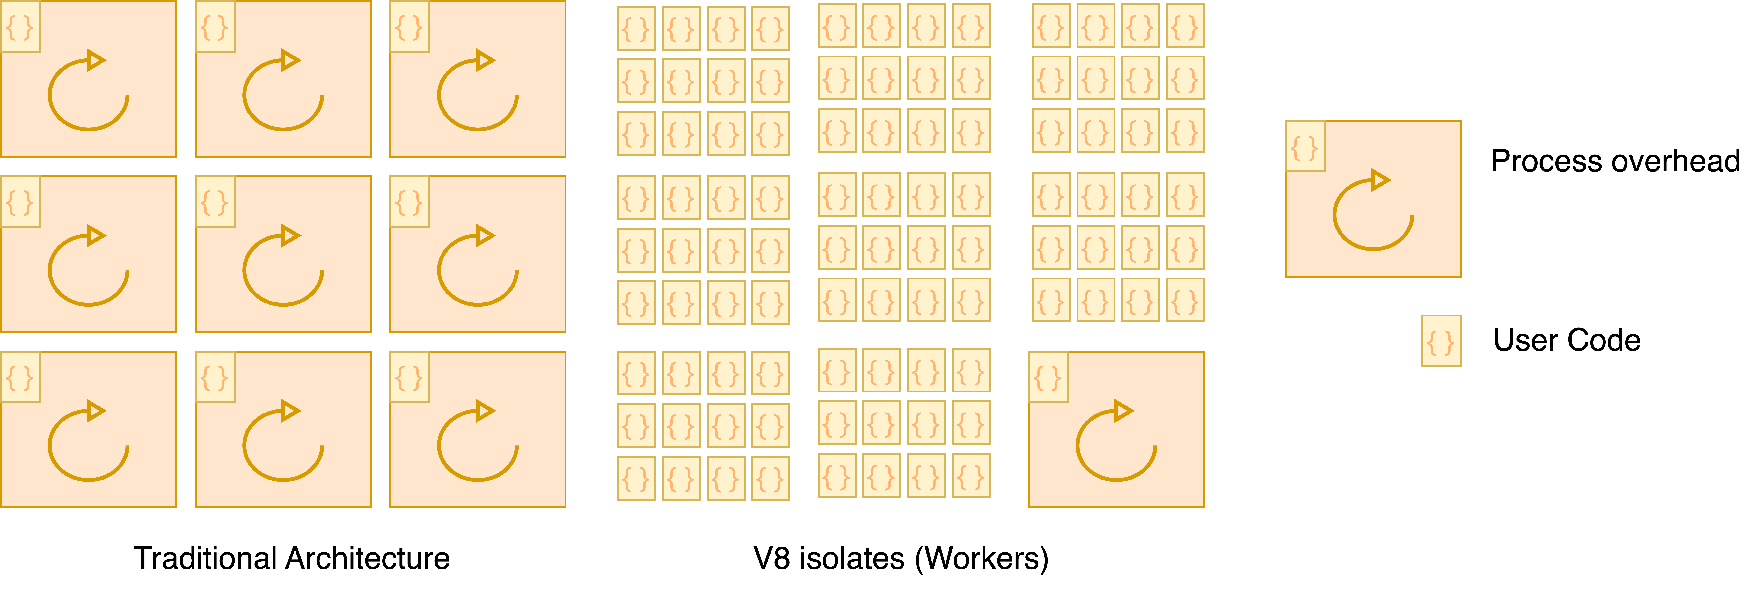
\includegraphics[width=\textwidth,height=\textheight,keepaspectratio]{images/runtimes/v8-isolates.pdf}
	\caption{containerized vs. \gls{V8} \glspl{isolate} figure redrawn from \cite{cloudflareinc_2023_how}}
	\label{fig:v8-isolates}
\end{figure}

\subsection{Comparing V8 Isolates to WebAssembly Runtimes}

Both \gls{V8} isolates and WebAssembly are similar in the way that they both execute code in a sandboxed environment. However, a V8 isolate is a JavaScript powered worker, while WebAssembly on the other hand is a binary instruction format. On the bright side, a V8 engine can include a WebAssembly runtime, which means that a V8 based cloud providers will be able to support multiple languages through WebAssembly. 

When it comes to performance, according to Lin Clark's article on the release of Wasmtime \cite{clark_2022_wasmtime}, "a JS isolate startup time is about 5 milliseconds while a WebAssembly runtime startup time is about 50 microseconds. She then writes that WebAssembly is more lightweight and therefore, it can have many more instances running at the same time compared to other coarse-grained isolates". 

We will compare the performance of V8 isolates to the performance of WebAssembly runtimes in Chapter \ref{chap:evalution} and measure the startup time of both approaches. 

\section{Serverless Requirements}
\label{sec:serverless-requirements}

The following summary of requirements should be met by an ideal serverless runtime, therefore, we will use them as a guideline to evaluate the different runtimes. 
A serverless runtime should be able to:
%
\begin{enumerate}
	\item Ensure security and isolation between functions.
	\item Have a small footprint to reduce the startup time of functions, therefore, a small memory footprint and also fast startup time. 
	\item Integrate effortlessly with existing frameworks. 
	\item Support multiple programming languages but not less to the traditional serverless platforms. 
	\item Execute functions with a speed comparable to native speed.
	\item Have the capability to run on various instruction set architectures, including but not limited to \texttt{x86\_64} and \texttt{arm}.
	\item Handle large amount of I/O operations concurrently.
\end{enumerate}

\section{Execution Models and Performance Implications}
\label{sec:execution-models-and-performance-implications}

One of the most important aspects of WebAssembly is its versatility. WebAssembly can be used in a wide variety of use cases, from running in the browser to running on microcontrollers. However, the different use cases require different execution models. For example, in a serverless function, the WebAssembly module could be compiled and executed ahead of time. On the other hand, in a microcontroller, the WebAssembly module is preferably executed by a WebAssembly interpreter. 

Moreover, \gls{WebAssembly} supports many programming languages and runs on various instruction set architectures, because the specification is designed to be fast, secure and portable \cite{butcher_2023_the}. 

This section is dedicated to exploring the different execution models and how they influence the performance of the runtimes, so that we can evaluate and discuss the benchmark results in chapter \ref{chap:evalution}.

\subsection{Choice of Programming Languages}
\label{sec:programming-languages}

The choice of a programming language does affect the performance and the size of the WebAssembly module. System programming languages like C/C++ and Rust are lightweight and require little runtime overhead. On the other hand, languages like Java and .NET bring a lot of runtime overhead, which increases the size of the WebAssembly module \cite{butcher_2023_the}. % garbage collection proposal

\subsubsection{Compliler Code Optimization}
\label{sec:compliler-code-optimization}

Some compilers, like the Rust compiler, can utilize compiler flags to prioritize the quality of the output code over the compilation time. In case of Rust, the \texttt{opt-level} flag can be used to set the optimization level. The default value is \texttt{opt-level=0}, which means that the compiler will prioritize the compilation time over the quality of the output code. The highest value is \texttt{opt-level=3}, which means that the compiler will prioritize the quality of the output code over the compilation time. As a result, the output code will have a better execution performance and a smaller size \cite{rustlangcommunity_2021_customizing}. 

\subsection{JIT - Just In Time Compilation}
\label{sec:jit}

A Just In Time Compilation (JIT) is a technique in which WebAssembly module is compiled into native machine code when it's about to be executed. The code is optimized for the running hardware. The JIT compilation comes at the cost of a longer startup time compared to an Interpreter or Ahead of Time (AOT) compilation. This penalty is specially noticeable in smaller functions, where the execution time is short \cite{butcher_2023_the}. 

\subsection{Interpreter}
\label{sec:interpreter}

An interpreter runtime, such as Wasm3, processes and executes small chunks of code in sequence \cite{shymanskyy_2023_wasm3}. This execution model incurs minimal, if any, startup time penalty as it only uses resources when required. Furthermore, because it minimizes the workload, it has a small memory footprint, making it ideally suited for resource-constrained devices like microcontrollers. Notwithstanding, for long-running functions, its execution speed is generally slower compared to JIT-based runtimes \cite{butcher_2023_the}. 

\subsection{AOT - Ahead Of Time Compilation}
\label{sec:aot}

An Ahead of Time (AOT) compilation is a technique in which the WebAssembly module is compiled into native machine code before it's executed. The code is optimized for the running hardware, thus, it can only run on the specific machine they were compiled for. The AOT compilation comes at the cost of a longer build time compared to an Interpreter or JIT compilation. However, the AOT compilation has the advantage of a fast startup time and a fast execution time. Moreover, each runtime possesses its unique format for these optimizations, meaning for example a Wasmtime AOT-compiled program will not be compatible with other Wasm runtimes like Wasmer \cite{butcher_2023_the}. 

The Wasmtime runtime has the capability to compile a Wasm module into an AOT-compiled binary. For example, given we have a Wasm module called \texttt{myfunction.wasm}, we can compile it into an AOT-compiled binary \texttt{myfunction.cwasm} by running the following command \cite{bytecodealliance_2022_wasmtime}: \texttt{wasmtime compile myfunction.wasm}

The performance benefits of AOT compilation are likely noticeable on long-running complex functions outperforming JIT compilation.

Nonetheless, the compiled binaries are larger than the original Wasm modules, due to the fact that many of the optimizations are incorporated into the binary. This is a trade-off between the size of the binary and the performance of the function. 
% too much opinionated
In regards to serverless functions, the AOT compilation model is the most suitable, because it has a fast startup time and a fast execution time. Moreover, the drawbacks namely the larger binary size can be neglected, because the serverless functions are usually small in size and the portability of the Wasm modules is not a concern, because the functions can be compiled for the specific machine on deployment phase.

\subsection{Wasm Snapshots (Wizer)}
\label{sec:wizer}

As noted earlier, for \gls{serverless} functions, having a fast startup time is crucial. 
Thus, techniques that can remove the repetitive initialization step from the critical 
path are highly beneficial. Wizer is a tool that can create a snapshot of an already 
initialized WebAssembly module. The snapshot is a pre-initialized Wasm module that should start 
faster without sacrificing any security or portability. 

As shown in Figure \ref{fig:wizer}, a program needs to go through four phases before it can be executed. 
The steps can be divided into two sections - the time of the developer spends to build and upload the program and the time of the user waiting for the program to become interactive on each request. The user experience can be enhanced by reducing the time spent in the second section. 

\begin{figure}[H]
	\centering
	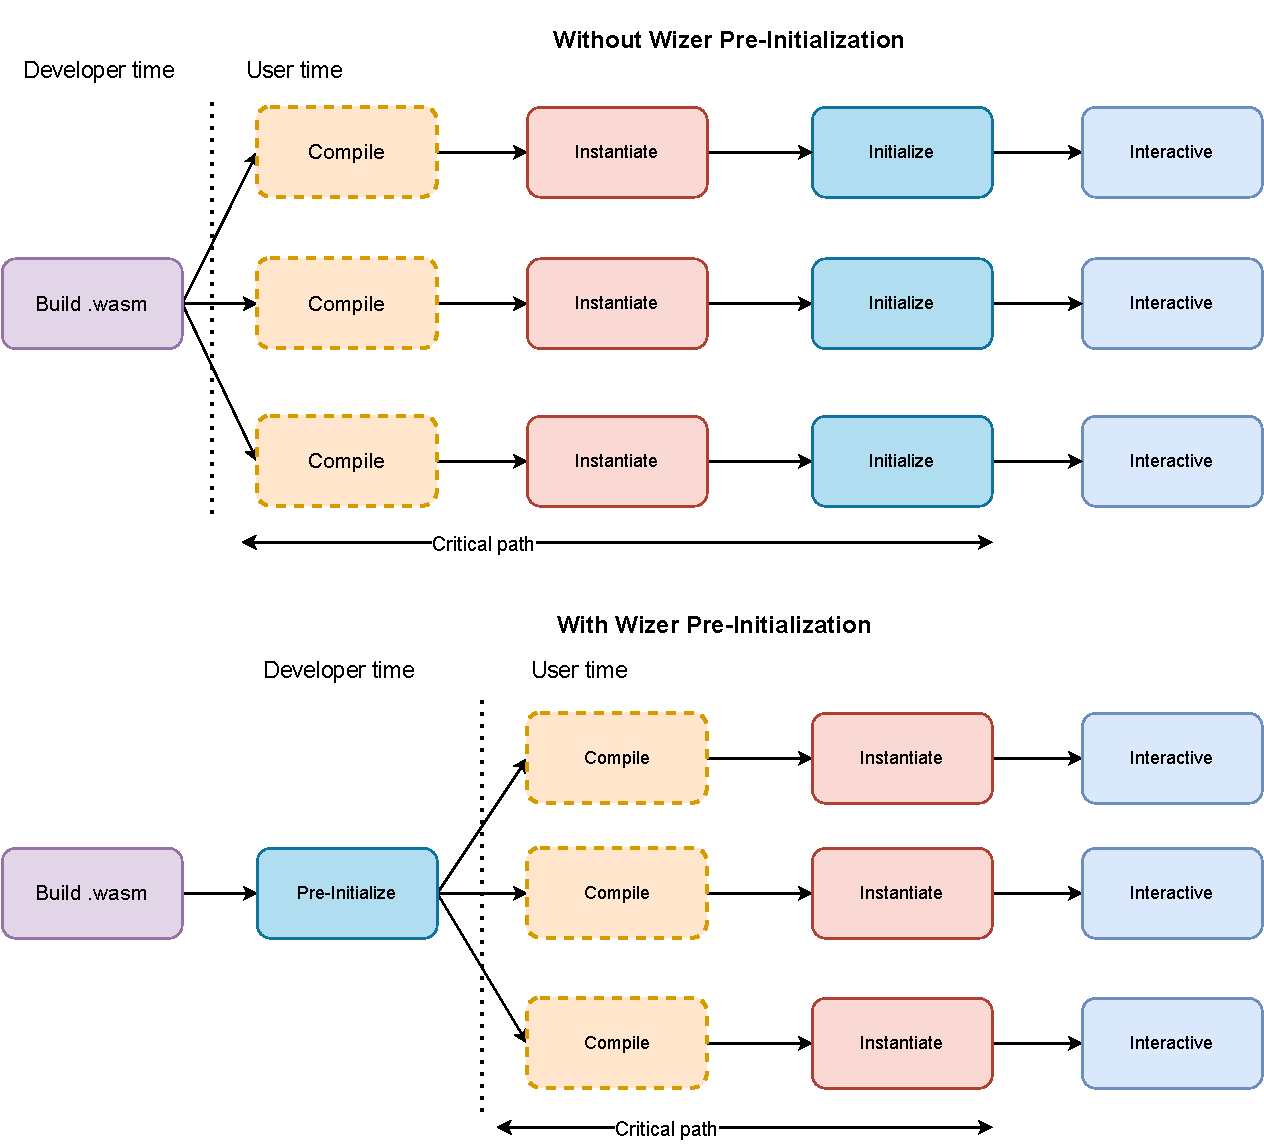
\includegraphics[width=1\linewidth]{images/runtimes/Wizer.drawio.pdf}
	\caption{Overview of Pre-initialization vs. Non Pre-initialization, based on \cite{fitzgerald_2021_hit}}
	\label{fig:wizer}
\end{figure}

Wizer creates a pre-initialized snapshot through these four phases \cite{fitzgerald_2021_hit}:
\begin{enumerate}
	\item Instrument: The first phase, known as the instrumentation phase, aims to export the internal state of the Wasm module so that Wizer can read it during the snapshot phase.
	\item Initialize: In the second phase, Wizer uses the Wasmtime runtime to compile and initialize the Wasm module. It then calls the exported "wizer.initialize" function.
	\item Snapshot: The third phase is the snapshot phase, in which Wizer reads the exports created in the first phase and generates the snapshot structure.
	\item Rewrite: The final phase is the rewrite phase. Wizer takes the initial Wasm module and the snapshot to create a new Wasm module. It removes the start section, as the snapshot has already executed the initializations, and updates each memory's minimum size to the size of the snapshot memories, as they may have grown during the initialization phase.
\end{enumerate}


\subsubsection{Wizer benchmarks}
\label{sec:wizer-benchmarks}

Initial benchmarks indicate that Wizer can provide between 1.35 and 6.00 times faster instantiation and initialization, depending on the specific workload. Running the benchmarks included in the Wizer repository \cite{bytecodealliance_2023_wizer}, we can confirm that Wizer can provide a significant speedup in the instantiation and initialization phases. For \ref{fig:uap-bench} we ran the User Agent Parsing benchmark from the Wizer repository. The benchmark creates a "RegexSet" using user agent parsing regexes from the Browserscope project. Then, it tests if the input string matches any known user agent patterns. 

The results on the User Agent Benchmark shows 14 times faster instantiation more than double the speedup of the original benchmark. We used the newest version of Wizer and Wasmtime ran on a M1 Pro MacBook with 32GB of RAM.

However, there is a caveat to this benchmark, it is important to note that not all programs will experience enhancements in instantiation and startup latency. For instance, Wizer can frequently enlarge the Data section of a Wasm module, potentially leading to adverse effects on network transfer times for web applications. 

In the case of the User Agent Parsing benchmark, the orginal Wasm module is 3.1MB and the snapshot is 35.7MB. The size of the snapshot is 11.5 times larger than the original Wasm module. This is because the snapshot contains a large set of regexes in the data segment.
In the context of \gls{edge computing}, this could be a problem, as the larger the Wasm module, the longer it takes to transfer it to the edge hosts. Furthermore, both Cloudflare and Fastly cache the executable code across their global network of edge servers. Thus, making this solution on some instances less desirable. 

\begin{figure}[H]
	\centering
	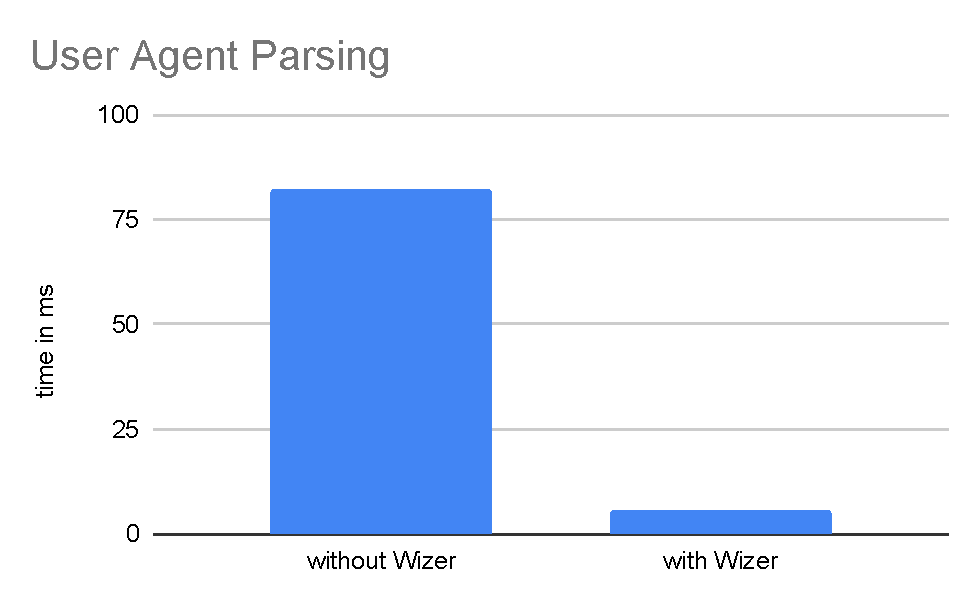
\includegraphics[width=0.6\linewidth]{images/runtimes/UAP.pdf}
	\caption{User Agent Parsing benchmark}
	\label{fig:uap-bench}
\end{figure}
